\section{Results and analysis}
\subsection{Order stability}
\label{sec:order-stability}
We first test whether the scoring interface preserves candidate identity under changes in presentation order. We compare three scoring interfaces, summarized in Table~\ref{tab:structural-properties}. Their inputs, candidate interactions, and readouts are defined as follows.

\textbf{Independent Pointer} removes the candidate-interaction blocks and scores each independently encoded candidate using a shared 256-dimensional query--key pointer. \textbf{Set Pointer} adds two position-free Transformer blocks (four heads, fourfold feed-forward expansion, GELU, zero dropout), with the query bypassing candidate interaction. \textbf{Complete-candidate LM} encodes all labeled alternatives together and normalizes next-token logits over their single-token labels. All interfaces directly output candidate probabilities; Table~\ref{tab:structural-properties} summarizes their structural properties.

\begin{table}[htbp]
\centering\small
\begin{tabular}{lcc}
\toprule
Interface & Candidate interaction & Equivariant scores \\
\midrule
Independent Pointer & No & Yes \\
Set Pointer & Yes & Yes \\
Complete-candidate LM & Yes & Not guaranteed \\
\bottomrule
\end{tabular}
\caption{Structural properties under the preprocessing and masking conditions in the method. Equivariance is a score property; ties and floating-point effects require separate decision-level checks.}
\label{tab:structural-properties}
\end{table}
For the complete-method checkpoints used in Table~\ref{tab:unified-standard}, LM changes its selected candidate on 108 of 755 questions (14.30\%) across exhaustive permutations; Set changes on none. Each question is evaluated under all 24 candidate orders, yielding 18,120 predictions per model. Predictions are aligned by candidate identity before comparison. Figure~\ref{fig:decision-analysis} connects this order stability to the complete-method performance under larger difficult candidate sets.




\subsection{Candidate interaction enables preference reversals}
Paired three-choice questions share two objects but replace the third with a smaller or larger extreme, reversing the correct median. Candidate-independent utilities cannot reverse the shared objects' ranking. We test fixed checkpoints on 512 fresh scenes (2,048 questions), averaging three training seeds; a largest-object task controls for ordinary ranking.
\begin{table}[htbp]
\centering\small
\begin{tabular}{lrrrrr}
\toprule
& \multicolumn{3}{c}{Median relation} & \multicolumn{2}{c}{Maximum control} \\
Model & Acc. (\%) & Pairs (\%) & NLL & Acc. (\%) & NLL \\
\midrule
Independent & 50.0000 & 0.0000 & 0.70072 & 99.7721 & 0.01175 \\
Set & 99.0234 & 98.3073 & 0.25971 & 99.5768 & 0.03669 \\
Complete LM & 99.7721 & 99.5443 & 0.01878 & 99.8372 & 0.01062 \\
\bottomrule
\end{tabular}
\caption{Fresh-scene test of fixed 80-epoch checkpoints, equally averaging the three retained training seeds. Pairs require both questions correct; all NLL values are uncalibrated. Set and complete-candidate LM both learn the median relation, which requires candidate interaction. The training budget is matched by optimizer updates.}
\label{tab:relation-duration-fresh}
\end{table}

Set resolves the median relation. Independent achieves 99.7721\% accuracy on the maximum control and 0.0000\% paired accuracy on preference reversals. The Set-minus-Independent median-pair difference is 98.3073 percentage points, with paired whole-scene interval $[97.4609,99.0234]$. The complete-candidate LM provides a second interaction-capable reference. The experiment demonstrates the role of candidate-dependent computation. The synthetic test reports raw probabilities.

\subsection{Standard recognition and candidate-count transfer}
\label{sec:unified-recognition}
We evaluate the complete decision model under matched balanced six-dataset training. Both interfaces use cross-entropy plus the dataset-wise calibration loss and a separately fitted temperature. Table~\ref{tab:unified-standard} reports one mixed-dataset model per interface, using the fixed final checkpoint from one shared training seed. Set reaches 90.35\% equal-dataset accuracy versus 90.09\% for LM, a difference of $+0.2690$ percentage points with paired interval $[+0.0086,+0.5317]$.
\begin{table}[htbp]
\centering\small
\begin{tabular}{lrrr}
\toprule
Dataset & LM (\%) & Set (\%) & Difference (pp) \\
\midrule
Pets & 95.88 & 95.42 & -0.46 \\
CUB & 84.52 & 85.57 & +1.05 \\
Cars & 93.74 & 93.83 & +0.09 \\
Dogs & 85.65 & 85.80 & +0.15 \\
Flowers & 99.11 & 98.99 & -0.11 \\
Aircraft & 81.61 & 82.51 & +0.90 \\
\midrule
Equal-dataset mean & 90.09 & 90.35 & +0.27 \\
\bottomrule
\end{tabular}
\caption{Unified mixed-dataset models on author-defined four-choice test records, using the same shuffled candidate sets for both methods. Each method uses one balanced CE-plus-calibration checkpoint across all six datasets, followed by its own held-out temperature. One training seed; differences are Set minus LM, computed before rounding.}
\label{tab:unified-standard}
\end{table}

\paragraph{Transfer to larger difficult candidate sets.}
We evaluate these same complete-method checkpoints at candidate counts of two, four, ten, and twenty, keeping the class inventory fixed. Distractors are selected by the recorded image--text ranking. Table~\ref{tab:full-method-hard} reports equal-dataset accuracy. The Set--LM gap is +0.44 percentage points at four candidates (paired 95\% interval $[+0.17,+0.70]$) and +1.80 points at twenty candidates ($[+1.42,+2.20]$). The larger difficult sets therefore expose a stronger accuracy advantage for Set within this evaluation, while the model is trained with four candidates.
\begin{table}[htbp]
\centering\small
\begin{tabular}{rrrr}
\toprule
Candidates & LM (\%) & Set (\%) & Difference (pp) \\
\midrule
2 & 93.47 & 93.85 & +0.38 \\
4 & 90.10 & 90.54 & +0.44 \\
10 & 84.62 & 86.00 & +1.38 \\
20 & 80.26 & 82.06 & +1.80 \\
\bottomrule
\end{tabular}
\caption{Difficult-candidate count transfer of the complete-method checkpoints in Table~\ref{tab:unified-standard}. Training uses four candidates; test candidates are mined with the fixed image--text ranking. Values are six-dataset mean accuracies from one shared training seed. Differences are Set minus LM.}
\label{tab:full-method-hard}
\end{table}

\subsection{Training with variable candidate counts}
\label{sec:dynamic-k-training}
We test how exposure to variable candidate counts affects performance on larger decision sets. We train each interface with a candidate count sampled independently and uniformly from $K\in\{2,4,10\}$ for each image and epoch. Image exposure, optimizer updates, backbone and development-selection rule are held fixed; the standard four-choice development set still selects the checkpoint. Candidate-token computation varies with the sampled count. The test candidate sets are identical across all four checkpoints, and twenty candidates remain outside the training support. The category inventory is held fixed while candidate count varies.
\begin{table}[htbp]
\centering\small
\begin{tabular}{lrrrr}
\toprule
Test & LM fixed & Set fixed & LM variable & Set variable \\
\midrule
Standard & 89.08 & 89.79 & 89.08 & 89.82 \\
Hard 2 & 92.87 & 93.36 & 92.73 & 93.26 \\
Hard 4 & 89.25 & 89.93 & 89.13 & 89.91 \\
Hard 10 & 84.94 & 86.27 & 86.02 & 87.24 \\
Hard 20 & 82.01 & 84.47 & 84.20 & 85.82 \\
\bottomrule
\end{tabular}
\caption{Equal-dataset accuracy (\%) for fixed four-candidate training and variable-candidate training. All four models use the same single training seed and test records. Difficult-distractor tests and the author-defined standard test are separate constructions.}
\label{tab:dynamic-k-training}
\end{table}
At twenty difficult candidates, the change from fixed to variable training is +2.19 [+1.86, +2.53] percentage points for LM and +1.35 [+1.08, +1.62] for Set (paired image-bootstrap intervals). The corresponding change in the Set--LM gap is -0.85 [-1.25, -0.45] percentage points. These comparisons condition on the selected weights and assess the variable-count training recipe, including its candidate-token computation.
Both methods improve at larger difficult candidate counts, but LM benefits more at twenty candidates, narrowing the Set--LM gap. Set retains a positive gap of +1.62 [+1.31, +1.93] percentage points after variable-count training. Thus the magnitude of the fixed-count advantage depends partly on training exposure. Standard-test point estimates remain close to their fixed-count counterparts. On the same exhaustive-order subset, the variable-count Set still has no decision changes, whereas the variable-count LM still changes candidate identity. The permutation test distinguishes the order behavior of the two interfaces after variable-count training.


\subsection{Training and post-training calibration}
Table~\ref{tab:unified-probability} evaluates the probability outputs of the complete-method checkpoints. Independently fitted temperatures reduce NLL and Brier for both interfaces while preserving their decisions. After calibration, Set has NLL 0.2831 versus 0.2778 for LM; the paired Set-minus-LM difference is $+0.00530$ with interval $[+0.00004,+0.01054]$. Set has a lower Brier point estimate, 0.1428 versus 0.1438, with difference $-0.00105$ and interval $[-0.00356,+0.00148]$. Figure~\ref{fig:calibration-analysis} visualizes how temperature scaling changes the confidence--accuracy relationship within each dataset.
\begin{table}[htbp]
\centering\small
\begin{tabular}{lrrrr}
\toprule
& \multicolumn{2}{c}{Raw} & \multicolumn{2}{c}{Temperature-scaled} \\
\cmidrule(lr){2-3}\cmidrule(lr){4-5}
Metric $\downarrow$ & LM & Set & LM & Set \\
\midrule
NLL & 0.3008 & 0.3478 & 0.2778 & 0.2831 \\
Sum-Brier & 0.1473 & 0.1480 & 0.1438 & 0.1428 \\
ECE & 0.0337 & 0.0448 & 0.0224 & 0.0355 \\
\bottomrule
\end{tabular}
\caption{Equal-dataset mean probability metrics for the balanced CE-plus-calibration checkpoints in Table~\ref{tab:unified-standard}. ECE uses fifteen equal-count bins and is descriptive. Lower is better. Calibration uses post-training temperature scaling.}
\label{tab:unified-probability}
\end{table}


\begin{figure}[htbp]
\centering
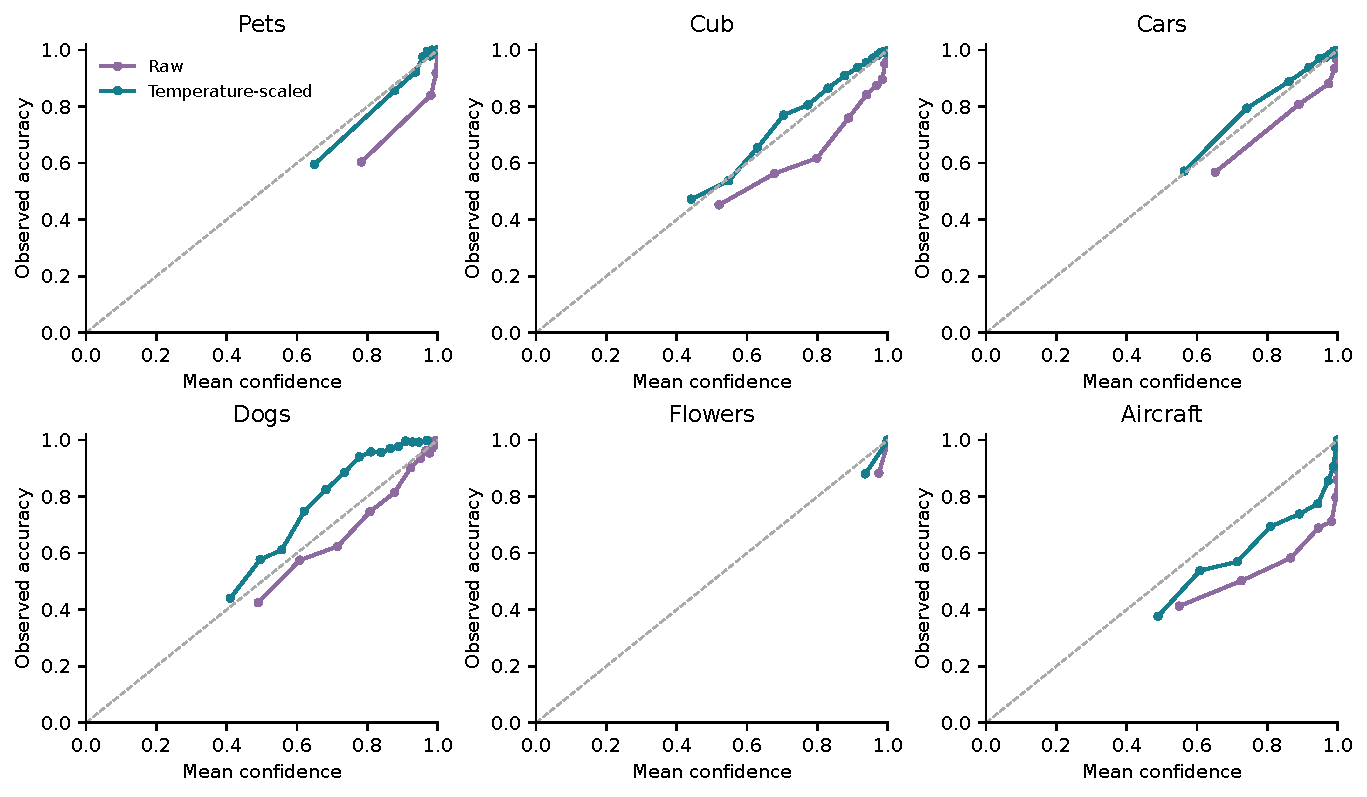
\includegraphics[width=\linewidth]{../figures/calibration-analysis.pdf}
\caption{Probability calibration of the complete Set model on the six recognition datasets. Each curve uses fifteen equal-count confidence bins; points show mean top-choice confidence and observed accuracy. The dashed diagonal denotes matched confidence and accuracy. Temperature scaling uses the single scalar fitted on the reserved calibration data, with unchanged predictions.}
\label{fig:calibration-analysis}
\end{figure}

\paragraph{Training-time calibration.}
We further compare cross-entropy training with a dataset-wise mean-confidence penalty under a matched, balanced six-dataset training recipe. Both Set models use the same seed, candidate exposures, and final-epoch checkpoint. Table~\ref{tab:training-calibration} shows that the penalty improves raw NLL, Brier, and ECE while changing macro accuracy from 90.48\% to 90.35\%. Fitting a separate temperature for each model by minimizing equal-dataset calibration NLL further improves probability quality: NLL decreases from 0.2985 to 0.2831 and Brier from 0.1457 to 0.1428 when the training penalty is added. The paired NLL difference is $-0.01539$ with interval $[-0.01953,-0.01142]$; the accuracy difference is $-0.1273$ percentage points with interval $[-0.3205,+0.0676]$. These results support combining the training penalty with post-training temperature scaling. Appendix~\ref{sec:training-calibration-protocol} specifies the matched training recipe.
\begin{table}[htbp]
\centering\small
\begin{tabular}{llrrrr}
\toprule
Training & Probability & Accuracy (\%) & NLL $\downarrow$ & Brier $\downarrow$ & ECE $\downarrow$ \\
\midrule
CE & Raw & 90.48 & 0.4003 & 0.1519 & 0.0521 \\
CE + calibration & Raw & 90.35 & 0.3478 & 0.1480 & 0.0448 \\
CE & Temperature & 90.48 & 0.2985 & 0.1457 & 0.0427 \\
CE + calibration & Temperature & 90.35 & 0.2831 & 0.1428 & 0.0355 \\
\bottomrule
\end{tabular}
\caption{Training-loss comparison for Set under balanced six-dataset training with one shared seed. Metrics are equal-dataset means on the standard test; Brier is summed over candidates and ECE uses fifteen equal-count bins. Each model receives its own held-out temperature fitted with an equal-dataset NLL objective. Positive scalar temperature scaling preserves accuracy.}
\label{tab:training-calibration}
\end{table}


\subsection{Natural VQA performance}
On A-OKVQA, Set remains close to the native LM, with an accuracy decrease of 0.53 points across three seeds (Table~\ref{tab:vqa-native-summary}; exploratory interval $[-1.7041,0.6406]$). Scaled probability losses favor LM. This test evaluates retention of general VQA capability; split and uncertainty details are in Appendix~\ref{app:essential}.
\begin{table}[htbp]
\centering\small
\begin{tabular}{lrrr}
\toprule
Interface & Accuracy (\%) & Scaled NLL & Scaled Brier \\
\midrule
Native LM & 87.2800 & 0.3703 & 0.1845 \\
Set & 86.7495 & 0.3819 & 0.1932 \\
\bottomrule
\end{tabular}
\caption{Natural VQA capability and calibrated probability quality, using the completed supervised holdout experiment. Means use all registered seeds and frozen, independently fitted temperatures. The comparison follows the registered native-LM secondary analysis. Raw probability differences and protocol details appear in Appendix~\ref{app:essential}.}
\label{tab:vqa-native-summary}
\end{table}

